\documentclass[12pt, a4paper]{article}
\usepackage[utf8]{inputenc}
% \usepackage[russian]{babel}
\usepackage[pdftex]{graphicx, color}
\usepackage{amsmath, amsfonts, amssymb, amsthm}
\usepackage{bm}
\usepackage[left=2cm,right=2cm,top=1.5cm,bottom=2cm]{geometry}
\usepackage{indentfirst}
\usepackage{hyperref}
\usepackage{float}
\usepackage[table,xcdraw]{xcolor}
\usepackage{tikz}
\usepackage[justification=centering,labelfont=bf]{caption}
\usepackage{multirow}
\usepackage[normalem]{ulem}
\useunder{\uline}{\ul}{}
\usetikzlibrary{quotes,arrows.meta}

\graphicspath{{pics/}}

\begin{document}
    \begin{center}
        
\includegraphics[height=3cm]{UVM}

        {\large\textbf{
            CS352 Evolutionary Computation: Homework 2
        }}

        \vspace{0.3cm}

        \textit{\textbf{Ayat Ospanov}}

        \today
    \end{center}

    \tableofcontents

    \section{Question 1}
        The equation for the basic Schema Theorem is the next:
        \begin{align*}
            E[m(H, t+1)] \geq m(H, t) \frac{f(H)}{\bar{f}} \Big(1 - \frac{\delta(H)}{L - 1}p_c - o(H) p_m\Big)
        \end{align*}
        where
        \begin{itemize}
            \item $m(H, t)$ is the proportion of individuals representing schema H at time-step $t$
            \item $f(H)$ is the fitness of the schema H
            \item $\bar{f}$ is the mean fitness of the population
            \item $o(H)$ is the order of the schema H
            \item $\delta(H)$ is the defining length of the schema H
            \item $L$ is the length of a genotype
            \item $p_c$ is the probability of applying crossover
            \item $p_m$ is the bitwise mutation probability
        \end{itemize}

        The first factor $m(H, t) \frac{f(H)}{\bar{f}}$ is the probability of a
        schema being selected. It is obvious that it depends on the relative fitness
        of the schema (because the selection is fitness proportionate) and on the
        proportion of individuals.

        The second factor $1 - \frac{\delta(H)}{L - 1} p_c - o(H) p_m$ is the
        probability of surviving variation operators. $\frac{\delta(H)}{L - 1} p_c$
        is the probability of disrupting examples by crossover and $o(H) p_m$ is the
        probability of disrupting examples by mutation.

        Thus, the theorem states ``short, low-order (derives from the second factor)
        schemata with above-average fitness (the first factor) increase exponentially
        over generations''

    \section{Question 2}
        The fundamental message of the Schema Theorem, or Building Block Hypothesis,
        is that GAs can begin by selecting short, low-order schemata examples, and
        then combine them to create higher order schemata, repeating until a schema
        of length $L-1$ and order $L$ is created and selected.

    \section{Question 3}
        There are 3 types of problem ``difficulty''.
        \begin{itemize}
            \item intra-BB
            \item inter-BB
            \item extra-BB
        \end{itemize}
        The most important is an intra-BB difficulty, or deceptiveness. This means
        at least one optimal schema is outcompeted by non-optimal schema.

    \section{Question 4}
        \begin{align*}
            S1 &= \texttt{*0**11***0**}, & o(S1) = 4, \delta(S1) = 8, L = 12\\
            S2 &= \texttt{*****0*1****}, & o(S1) = 2, \delta(S1) = 2, L = 12
        \end{align*}

        {\bf a)} The probability $p_s$ of surviving both crossover and mutation is
        $$p_s(H) = (1 - p_m)^{o(H)}\Big(1 - p_c \frac{\delta(H)}{L - 1}\Big)$$

        Thus,
        \begin{align*}
            p_s(S1) &= (1 - p_m)^4 (1 - \frac{8 p_c}{11})\\
            p_s(S2) &= (1 - p_m)^2 (1 - \frac{2 p_c}{11})
        \end{align*}

        It is obvious, that $p_s(S1) \leq p_s(S2)$. And the probability of
        surviving of both of them is $p_s(S1) \cdot p_s(S2)$

        {\bf b)} As we know, ``building blocks'' are short (in terms of defining
        length) and low-order schematas. $S1$ cannot be called a ``building
        block'' as its order and length are high, while $S2$ can be called
        a ``building block'', because it has the length of 2 and the order
        of 2 which makes possible to describe $S2$ as short and low-order
        schemata.

    \section{Question 5}
        \begin{table}[H]
        \centering
            \begin{tabular}{ll}
            \rowcolor[HTML]{C0C0C0}
            string & fitness \\
            100    & 10      \\
            111    & 20      \\
            011    & 15      \\
            010    & 15
            \end{tabular}
        \end{table}

        {\bf a)}
        \begin{align*}
            f(1**) &= \frac{N_{100} f_{100} + N_{111} f(111)}{N_{100} + N_{111}} =\\
            &= \frac{25 * 10 + 25 * 20}{25 + 25} = \frac{10 + 20}{2} = 15
        \end{align*}

        {\bf b)}
        The estimated number of samples of a schemata H at the next step is:
        $$n(H, t+1) = n(H, t) \frac{f(H)}{\bar{f}}$$
        Thus, for the schemata \texttt{1**} we can get the estimated number of samples
        on the next step:
        $$n(\texttt{1**}, t+1) = 50 * \frac{15}{15} = 50$$

        But we need the estimated fitness. To count, we need to estimate the number
        of survivors of guys from the schema \texttt{1**}. As we know those guys and can
        estimate numbers for a scheme, we can put $H_1 = 100$ and $H_2 = 111$. Now
        let's estimate the numbers:
        \begin{align*}
            n(100, t+1) &= n(100, t) \frac{f(100)}{\bar{f}} = 25 \cdot \frac{10}{15} = 25 \cdot \frac{2}{3}\\
            n(111, t+1) &= n(111, t) \frac{f(111)}{\bar{f}} = 25 \cdot \frac{20}{15} = 25 \cdot \frac{4}{3}
        \end{align*}

        Now we can estimate the fitness value for the \texttt{1**} scheme.
        \begin{align*}
            f_{t+1}(\texttt{1**}) &= \frac{n(100, t+1) * f(100) + n(111, t+1) * f(111)}{n(100, t+1) + n(111, t+1)} =\\
            &= \frac{25 \cdot \frac{2}{3} \cdot 10 + 25 \cdot \frac{4}{3} \cdot 20}{50}
            = \frac{\frac{2}{3} \cdot 10 + \frac{4}{3} \cdot 20}{2} =\\
            &= \frac{10 + 2 \cdot 20}{3} = \frac{100}{6} \approx 16.7\\
        \end{align*}

    \section{Question 6}
        \begin{table}[H]
        \centering
            \begin{tabular}{|l|l|llllllll|}
            \hline
            \multicolumn{2}{l|}{phenotype (integer)} & 0   & 1   & 2   & 3   & 4   & 5   & 6   & 7   \\ \hline
            \multirow{2}{*}{genotype}    & binary    & 000 & 001 & 010 & 011 & 100 & 101 & 110 & 111 \\
                                         & gray      & 000 & 001 & 011 & 010 & 110 & 111 & 101 & 100 \\ \hline
            \multicolumn{2}{|l|}{fitness}             & 7   & 5   & 3   & 9   & 10  & 1   & 6   & 6   \\ \hline
            \end{tabular}
        \end{table}

        \begin{table}[H]
        \centering
        \caption{Schema Analysis for binary code and gray code}
        \label{tab:sa}
            \begin{tabular}{|l|l|c|ccc|ccc|c|}
            \hline
                                    & order   & 3          & \multicolumn{3}{c|}{2}                 & \multicolumn{3}{c|}{1}                 & 0              \\ \hline
            \multicolumn{10}{|c|}{} \\ \hline
            \multirow{8}{*}{binary} & schema  & 111        & 11*        & 1*1        & *11          & **1          & *1*        & 1**        & ***            \\
                                    & fitness & \textbf{6} & \textbf{6} & 3.5        & 7.5          & 5.25         & \textbf{6} & 5.75       & \textbf{5.875} \\ \cline{2-10}
                                    & schema  &            & 01*        & 0*1        & *01          & **0          & *0*        & 0**        &                \\
                                    & fitness &            & \textbf{6} & 7          & 3            & \textbf{6.5} & 5.75       & \textbf{6} &                \\ \cline{2-10}
                                    & schema  &            & 10*        & 1*0        & *10          &              &            &            &                \\
                                    & fitness &            & 5.5        & \textbf{8} & 4.5          &              &            &            &                \\ \cline{2-10}
                                    & schema  &            & 00*        & 0*0        & *00          &              &            &            &                \\
                                    & fitness &            & \textbf{6} & 5          & \textbf{8.5} &              &            &            &                \\ \hline
            \multicolumn{10}{|c|}{} \\ \hline
            \multirow{8}{*}{gray}   & schema  & 100        & 10*        & 1*0        & *10          & 0**          & *0*        & **0        & ***            \\
                                    & fitness & \textbf{6} & \textbf{6} & \textbf{8} & \textbf{9.5} & \textbf{6}          & \textbf{6} & \textbf{8} & \textbf{5.875} \\ \cline{2-10}
                                    & schema  &            & 11*        & 1*1        & *11          & 1**          & *1*        & **1        &                \\
                                    & fitness &            & 5.5        & 3.5        & 2            & 5.75   & 5.75       & 3.75       &                \\ \cline{2-10}
                                    & schema  &            & 01*        & 0*1        & *01          &              &            &            &                \\
                                    & fitness &            & \textbf{6} & 4          & 5.5          &              &            &            &                \\ \cline{2-10}
                                    & schema  &            & 00*        & 0*0        & *00          &              &            &            &                \\
                                    & fitness &            & \textbf{6} & \textbf{8} & 6.5 &              &            &            &                \\ \hline
            \end{tabular}
        \end{table}

        \begin{figure}[H]
            \centering
            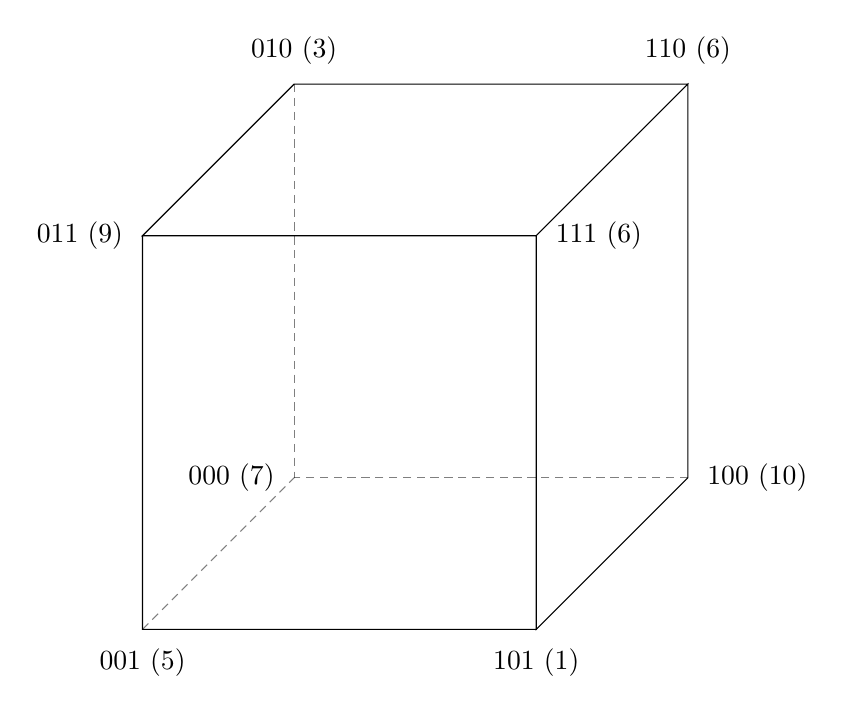
\begin{tikzpicture}[every edge quotes/.append style={auto, text=blue}]
                \pgfmathsetmacro{\cubex}{5}
                \pgfmathsetmacro{\cubey}{5}
                \pgfmathsetmacro{\cubez}{5}
                \draw [draw=black, every edge/.append style={draw=black, densely dashed, opacity=.5}]
                    (0,0,0) coordinate (o) -- ++(-\cubex,0,0) coordinate (a) -- ++(0,-\cubey,0) coordinate (b) edge coordinate [pos=1] (g) ++(0,0,-\cubez)  -- ++(\cubex,0,0) coordinate (c) -- cycle
                    (o) -- ++(0,0,-\cubez) coordinate (d) -- ++(0,-\cubey,0) coordinate (e) edge (g) -- (c) -- cycle
                    (o) -- (a) -- ++(0,0,-\cubez) coordinate (f) edge (g) -- (d) -- cycle;
                \node[label=right:111 (6)] at (o) {};
                \node[label=left:011 (9)] at (a) {};
                \node[label=below:001 (5)] at (b) {};
                \node[label=below:101 (1)] at (c) {};
                \node[label=above:110 (6)] at (d) {};
                \node[label=right:100 (10)] at (e) {};
                \node[label=above:010 (3)] at (f) {};
                \node[label=left:000 (7)] at (g) {};
            \end{tikzpicture}
            \caption{Hamming cube diagram for binary encoding}
            \label{fig:hamm_bin}
        \end{figure}

        \begin{figure}[H]
            \centering
            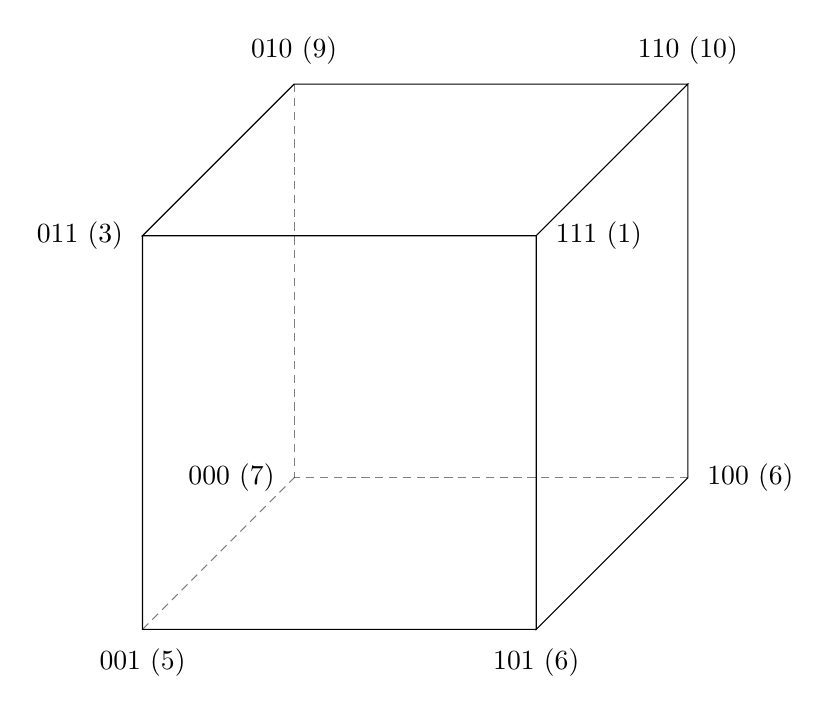
\begin{tikzpicture}[every edge quotes/.append style={auto, text=blue}]
                \pgfmathsetmacro{\cubex}{5}
                \pgfmathsetmacro{\cubey}{5}
                \pgfmathsetmacro{\cubez}{5}
                \draw [draw=black, every edge/.append style={draw=black, densely dashed, opacity=.5}]
                    (0,0,0) coordinate (o) -- ++(-\cubex,0,0) coordinate (a) -- ++(0,-\cubey,0) coordinate (b) edge coordinate [pos=1] (g) ++(0,0,-\cubez)  -- ++(\cubex,0,0) coordinate (c) -- cycle
                    (o) -- ++(0,0,-\cubez) coordinate (d) -- ++(0,-\cubey,0) coordinate (e) edge (g) -- (c) -- cycle
                    (o) -- (a) -- ++(0,0,-\cubez) coordinate (f) edge (g) -- (d) -- cycle;
                \node[label=right:111 (1)] at (o) {};
                \node[label=left:011 (3)] at (a) {};
                \node[label=below:001 (5)] at (b) {};
                \node[label=below:101 (6)] at (c) {};
                \node[label=above:110 (10)] at (d) {};
                \node[label=right:100 (6)] at (e) {};
                \node[label=above:010 (9)] at (f) {};
                \node[label=left:000 (7)] at (g) {};
            \end{tikzpicture}
            \caption{Hamming cube diagram for gray encoding}
            \label{fig:hamm_gray}
        \end{figure}

        {\bf b)} The problem is partially deceptive for both of encodings. For binary
        encoding the optimal schema 10* ($f(10*) = 5.5$) was outcompeted by non-optimal
        (e.g. $f(11*) = 6$), while the optimal schema 1*0 ($f(1*0) = 8$) outcompetes
        others. Thus, the problem for binary encoding is partially deceptive. For gray
        encoding the fitness value of the optimal schema 1*0 ($f(1*0) = 8$) is equal
        to the fitness value of the non-optimal schema 0*0 ($f(0*0) = 8$), which makes
        the problem partially deceptive.

        Now, to determine a type of deceptiveness, let's
        look at the Hamming diagrams. For binary encoding, we have maximum distance between
        suboptima ($f(011) = 9$) and the optima ($f(100) = 10$). That is binary encoded
        problem is Type II deceptive. Gray encoding has the minimum distance between sub-optima
        and optima. Thus, the problem in this case is Type I deceptive.

        {\bf c)} They are not. If we look at the columns for order 1 on the Table \ref{tab:sa},
        we can compute saliences for schemas as difference between corresponding rows. As in
        both encoding they have different differences, they are not uniformly scaled.

        {\bf d)} In case of non-uniformly scaled saliences, there is no selective pressure
        on lower order bits until the highest order bit gets fixed. Thus, it kills implicit
        parallelism, which makes it converge longer and it has so called domino convergence,
        when you drift from one suboptima to another step-by-step.

        {\bf e)} In terms of convergence, the gray encoding makes the problem easier as it
        becomes Type I deceptive. As we know, Type I deceptive problems are not GA-hard.
        On the other hand, Type II problem may converge faster, but it is not guaranteed
        it converges to the global optima. The convergence depends on parameters such as
        initial proportions of examples in population, etc.

        {\bf f)} The way to make an encoding to make the problem fully easy is arranging
        the fitness values ascending and assigning them to the Hamming cube's corners with the step
        of 1 in terms of the hamming distance. My custom encoding is given in the Table
        \ref{tab:cust_gt} and Fig. \ref{fig:hamm_custom}.

        \begin{table}[H]
        \centering
        \caption{Custom genotype}
        \label{tab:cust_gt}
            \begin{tabular}{|l|llllllll|}
            \hline
            phenotype       & 0   & 1   & 2   & 3   & 4   & 5   & 6   & 7   \\ \hline
            custom genotype & 100 & 011 & 101 & 010 & 110 & 001 & 000 & 111 \\ \hline
            fitness         & 7   & 5   & 3   & 9   & 10  & 1   & 6   & 6   \\ \hline
            \end{tabular}
        \end{table}

        \begin{figure}[H]
            \centering
            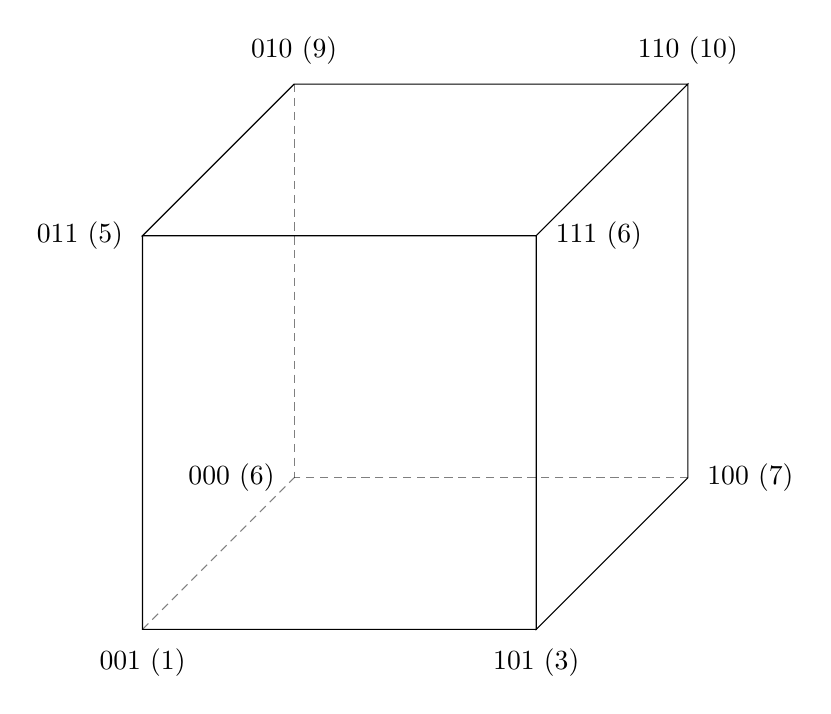
\begin{tikzpicture}[every edge quotes/.append style={auto, text=blue}]
                \pgfmathsetmacro{\cubex}{5}
                \pgfmathsetmacro{\cubey}{5}
                \pgfmathsetmacro{\cubez}{5}
                \draw [draw=black, every edge/.append style={draw=black, densely dashed, opacity=.5}]
                    (0,0,0) coordinate (o) -- ++(-\cubex,0,0) coordinate (a) -- ++(0,-\cubey,0) coordinate (b) edge coordinate [pos=1] (g) ++(0,0,-\cubez)  -- ++(\cubex,0,0) coordinate (c) -- cycle
                    (o) -- ++(0,0,-\cubez) coordinate (d) -- ++(0,-\cubey,0) coordinate (e) edge (g) -- (c) -- cycle
                    (o) -- (a) -- ++(0,0,-\cubez) coordinate (f) edge (g) -- (d) -- cycle;
                \node[label=right:111 (6)] at (o) {};
                \node[label=left:011 (5)] at (a) {};
                \node[label=below:001 (1)] at (b) {};
                \node[label=below:101 (3)] at (c) {};
                \node[label=above:110 (10)] at (d) {};
                \node[label=right:100 (7)] at (e) {};
                \node[label=above:010 (9)] at (f) {};
                \node[label=left:000 (6)] at (g) {};
            \end{tikzpicture}
            \caption{Hamming cube diagram for custom encoding}
            \label{fig:hamm_custom}
        \end{figure}

        The proof that the problem is fully easy is given in the Table \ref{tab:sa_custom}.
        Optimal schemas outcompete all non-optimal schemas. We have achieved it by constructing
        the encoding with no valleys.
        \begin{table}[H]
        \centering
        \caption{Schema Analysis for custom code. Optimal schemas are underscored.}
        \label{tab:sa_custom}
            \begin{tabular}{|l|l|c|ccc|ccc|c|}
            \hline
            {\color[HTML]{000000} }                         & {\color[HTML]{000000} order}   & {\color[HTML]{000000} 3}           & \multicolumn{3}{c|}{{\color[HTML]{000000} 2}}                                                                 & \multicolumn{3}{c|}{{\color[HTML]{000000} 1}}                                                                 & {\color[HTML]{000000} 0}              \\ \hline
            {\color[HTML]{000000} }                         & {\color[HTML]{000000} schema}  & {\color[HTML]{000000} 110}         & {\color[HTML]{000000} {\ul 11*}}  & {\color[HTML]{000000} 1*1}          & {\color[HTML]{000000} *11}          & {\color[HTML]{000000} **1}        & {\color[HTML]{000000} {\ul *1*}}    & {\color[HTML]{000000} {\ul 1**}}    & {\color[HTML]{000000} ***}            \\
            {\color[HTML]{000000} }                         & {\color[HTML]{000000} fitness} & {\color[HTML]{000000} \textbf{10}} & {\color[HTML]{000000} \textbf{8}} & {\color[HTML]{000000} 4.5}          & {\color[HTML]{000000} 5.5}          & {\color[HTML]{000000} 3.75}       & {\color[HTML]{000000} \textbf{7.5}} & {\color[HTML]{000000} \textbf{6.5}} & {\color[HTML]{000000} \textbf{5.875}} \\ \cline{2-10}
            {\color[HTML]{000000} }                         & {\color[HTML]{000000} schema}  & {\color[HTML]{000000} }            & {\color[HTML]{000000} 01*}        & {\color[HTML]{000000} 0*1}          & {\color[HTML]{000000} *01}          & {\color[HTML]{000000} {\ul **0}}  & {\color[HTML]{000000} *0*}          & {\color[HTML]{000000} 0**}          & {\color[HTML]{000000} }               \\
            {\color[HTML]{000000} }                         & {\color[HTML]{000000} fitness} & {\color[HTML]{000000} }            & {\color[HTML]{000000} 7}          & {\color[HTML]{000000} 3}            & {\color[HTML]{000000} 2}            & {\color[HTML]{000000} \textbf{8}} & {\color[HTML]{000000} 4.25}         & {\color[HTML]{000000} 5.25}         & {\color[HTML]{000000} }               \\ \cline{2-10}
            {\color[HTML]{000000} }                         & {\color[HTML]{000000} schema}  & {\color[HTML]{000000} }            & {\color[HTML]{000000} 10*}        & {\color[HTML]{000000} {\ul 1*0}}    & {\color[HTML]{000000} {\ul *10}}    & {\color[HTML]{000000} }           & {\color[HTML]{000000} }             & {\color[HTML]{000000} }             & {\color[HTML]{000000} }               \\
            {\color[HTML]{000000} }                         & {\color[HTML]{000000} fitness} & {\color[HTML]{000000} }            & {\color[HTML]{000000} 5}          & {\color[HTML]{000000} \textbf{8.5}} & {\color[HTML]{000000} \textbf{9.5}} & {\color[HTML]{000000} }           & {\color[HTML]{000000} }             & {\color[HTML]{000000} }             & {\color[HTML]{000000} }               \\ \cline{2-10}
            {\color[HTML]{000000} }                         & {\color[HTML]{000000} schema}  & {\color[HTML]{000000} }            & {\color[HTML]{000000} 00*}        & {\color[HTML]{000000} 0*0}          & {\color[HTML]{000000} *00}          & {\color[HTML]{000000} }           & {\color[HTML]{000000} }             & {\color[HTML]{000000} }             & {\color[HTML]{000000} }               \\
            \multirow{-8}{*}{{\color[HTML]{000000} custom}} & {\color[HTML]{000000} fitness} & {\color[HTML]{000000} }            & {\color[HTML]{000000} 3.5}        & {\color[HTML]{000000} 7.5}          & {\color[HTML]{000000} 6.5}          & {\color[HTML]{000000} }           & {\color[HTML]{000000} }             & {\color[HTML]{000000} }             & {\color[HTML]{000000} }               \\ \hline
            \end{tabular}
        \end{table}

    \section{Question 7}
        Let's assume we have done crossover and have $P_{ij}^{t+1}, i,j \in {0, 1}$.
        Now we do mutation for $P_{11}$: the number of samples that go to the next step
        is the number of samples which ``survive'' mutation. It is $(1 - p_m') P_{11}^{t+1}$,
        where $p_m' = 1 - (1 - p_m)^{o(H)}$ is the probability of destruction. Now
        calculate the constructive part. We can get $P_{11}$ from $P_{10}$ by flipping
        the second bit, from $P_{01}$ by flipping the first bit and from $P_{00}$ by
        flipping both bits. The probability of mutating only one bit is $p_m(1 - p_m)$.
        The equation means we flip one and don't flip the second. The probability of
        flipping both bits is $p_m^2$. Thus, we have the next equation for $P_{11}^{t+1}$:
        $$\mathbb{P}_{11}^{t+1} = (1 - p_m)^2 P_{11}^{t+1} + p_m(1 - p_m)[P_{01}^{t+1} + P_{10}^{t+1}] +
        p_m^2 P_{00}^{t+1}$$

        I put $\mathbb{P}$ to point out that that is the new value.

        Applying the same logic for others, we get the next set of equations:
        \begin{align*}
            \mathbb{P}_{00}^{t+1} &= (1 - p_m)^2 P_{00}^{t+1} + p_m(1 - p_m)[P_{10}^{t+1} + P_{01}^{t+1}] + p_m^2 P_{11}^{t+1} \\
            \mathbb{P}_{01}^{t+1} &= (1 - p_m)^2 P_{01}^{t+1} + p_m(1 - p_m)[P_{00}^{t+1} + P_{11}^{t+1}] + p_m^2 P_{10}^{t+1} \\
            \mathbb{P}_{10}^{t+1} &= (1 - p_m)^2 P_{10}^{t+1} + p_m(1 - p_m)[P_{11}^{t+1} + P_{00}^{t+1}] + p_m^2 P_{01}^{t+1} \\
            \mathbb{P}_{11}^{t+1} &= (1 - p_m)^2 P_{11}^{t+1} + p_m(1 - p_m)[P_{01}^{t+1} + P_{10}^{t+1}] + p_m^2 P_{00}^{t+1} \\
        \end{align*}

        To check the correctness of the system, we can sum the equations up and they should equal to 1:
        \begin{align*}
            Sum &= \mathbb{P}_{00}^{t+1} + \mathbb{P}_{01}^{t+1} + \mathbb{P}_{10}^{t+1} + \mathbb{P}_{11}^{t+1} = \\
            & = (1 - p_m)^2 [P_{00}^{t+1} + P_{01}^{t+1} + P_{10}^{t+1} + P_{11}^{t+1}] +\\
            & + 2 p_m (1 - p_m)[P_{00}^{t+1} + P_{01}^{t+1} + P_{10}^{t+1} + P_{11}^{t+1}] +\\
            & + p_m^2 [P_{00}^{t+1} + P_{01}^{t+1} + P_{10}^{t+1} + P_{11}^{t+1}] =\\
            & = \{as P_{00}^{t+1} + P_{01}^{t+1} + P_{10}^{t+1} + P_{11}^{t+1} = 1\} =\\
            & = (1 - p_m)^2 + 2 p_m (1 - p_m) + p_m^2 =\\
            & = [(1 - p_m) + p_m]^2 = 1
        \end{align*}\textbf{}

\end{document}
